\documentclass[12pt,a4paper]{article}  %klasa Marcina Wolińskiego
\usepackage[utf8]{inputenc}   
\usepackage[T1]{fontenc}
\usepackage[MeX,plmath]{polski} 
\usepackage{graphicx}
\usepackage[hidelinks]{hyperref}
\usepackage{xcolor}
\definecolor{myLightBlue}{RGB}{231, 240, 247}
\definecolor{myBlue}{RGB}{15, 106, 180}
\usepackage{fancyvrb}

\begin{document}
	\thispagestyle{empty}
	
		\begin{center}
			
			\centering

\includegraphics[keepaspectratio,scale=0.1]{./img/godlo.PNG} \\[.8cm]

			{\fontsize{17}{17}\selectfont
				\textsc{Politechnika Śląska \\[.3cm]
					Wydział Matematyki Stosowanej  \\[.3cm]
					Kierunek Informatyka  \\[2.5cm]}
				\textbf{Dokumentacja projektu \\[1.7cm]}}
			
			
			
			\large 
			{System zarządzania obowiązkami domowymi działający 
			w czasie rzeczywistym } \\[3.cm]

			
			\large
			\begin{flushleft}
				 Kamil Król, \\
			        Mateusz Ostalecki
			\end{flushleft}
			
			\vspace{3cm}
			Gliwice, styczeń 2020
		\end{center}

	\newpage
	\thispagestyle{empty}
	\tableofcontents
	\newpage
	
	\section{Wprowadzenie}
	\setcounter{page}{1}
		\subsection{Ogólny opis}
		Aplikacja jest systemem zarzadzania obowiązakami domowymi w formie\\ witryny internetowej. \\[0.5cm]
		Składa się ona z trzech głównych funkcjonalności:
		\begin{itemize}
			\item Strony logowania
			\item Strony rejestracji
			\item Strony panelu obsługi obowiązków
		\end{itemize}
		Strona logowania jest standardowym systemem autoryzacji dostepu do \\ głównego panelu. \\
		W celu zalogowania należy utworzyć konto w panelu rejestracji. \\
		Główny panel aplikacji posiada w sobie wszystkie funkcjonalosci pozwalające na zarzadzanie obowiązkami.\\
		\subsection{Linki do aplikacji}
		Działajacą aplikację można przetestować pod adresem: \\ \textcolor{blue}{\url{http://housework-client.herokuapp.com}} \\ [1.0cm]
		Adres serwera znajduje sie pod adresem: \\
		\textcolor{blue}{\url{http://housework-api.herokuapp.com/}} \\ [1.0cm]
		Kod źródłowy można znaleźć pod adresem: \\
		\textcolor{blue}{\url{https://github.com/KrolKamil/housework}} \\ [1.0cm]
	\newpage
	\section{Funkcjonalnośći aplikacji}
		\subsection{Logowanie}
		Logowanie wymaga podania nazwy użytkownika oraz hasła w celu \\ autoryzacji.
		Błędne wpisane hasło będzie skutkować podkreśleniem „inputu” na czerwono. \\
		Poprawnie zalogowany użytkownik zostanie przekierowany do głównego panelu.
		\begin{center}
			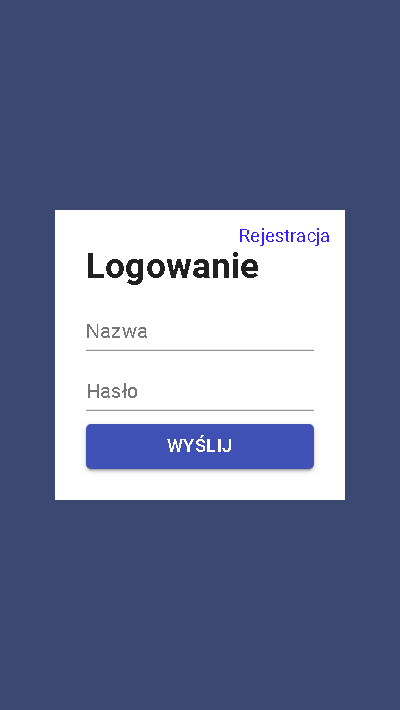
\includegraphics[keepaspectratio,scale=0.65]{./img/login.PNG} \\[.8cm]
		\end{center}
		\newpage
		\subsection{Rejestracja}
		Rejestracja wymaga podania nazwy użytkownika oraz hasła w celu rejestracji.
		Błędne wpisane hasło będzie skutkować podkreśleniem „inputu” na czerwono. \\
		Poprawnie zarejestrowany użytkownik zostanie przekierowany do głównego panelu.
		\begin{center}
			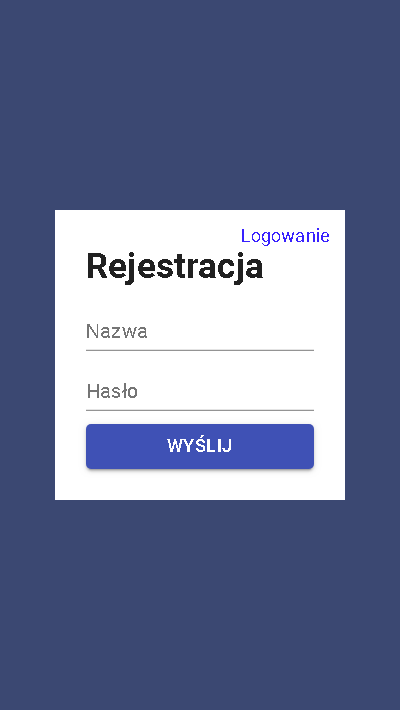
\includegraphics[keepaspectratio,scale=0.65]{./img/register.PNG} \\[.8cm]
		\end{center}
		\newpage
		\subsection{Panel Główny}
		\textbf{Panel główny posiada najważniejsze funkcjonalności aplikacji:}
		\subsubsection{Przegląd i manipulacja pozycjami zadań}
		W główym widoku widzimy wszystkie zdefiniowane zadania. \\
		Jasnoniebieski kolor posiadają zadania które możemy swobodnie przesówać pomiedzy kolumnami - są to zadania które jeszcze nikt nie rozpoczął lub czekają w kolumnie „DO ZROBIENIA”. \\
		Zadania w ostatniej kolumnie jeśli zostały wykonane przez nas mogą zostać usunięte przez przynisk „kosza”.\\
		
\includegraphics[keepaspectratio,scale=0.5]{./img/dashboard.PNG} 
		\subsubsection{Nowe zadanie}
		Po kliknięciu w przycisk „DODAJ ZADANIE” aplikacja przeniesie nas do okna dodawania nowego obowiązku. \\
		Pole z „Tytułem” jest wymagane zaś opis jest opcjonalny. \\
		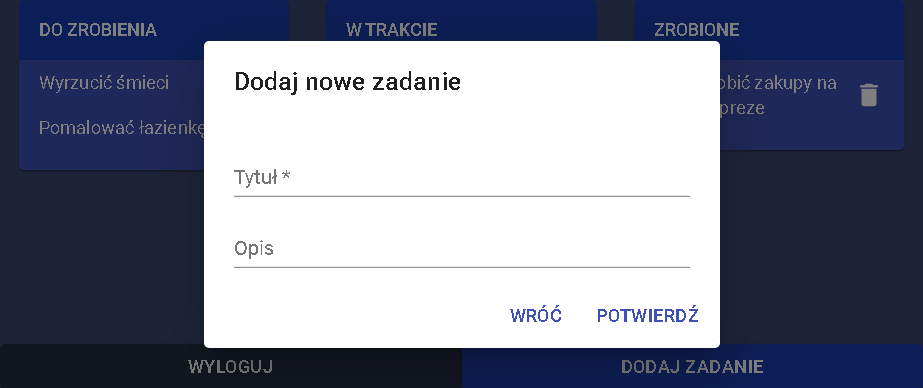
\includegraphics[keepaspectratio,scale=0.5]{./img/new.PNG} 
		\subsubsection{Edycja i podglad opisu zadania}
		Po kliknięciu w zadanie wyświetli nam sie okno w który możemy podejrzeć opis zadania i jesli zadanie znajduje sie w kolumnie „DO ZROBIENIA” lub my przenieśliśmy je na inna kolumne możemy je również edytować. \\
		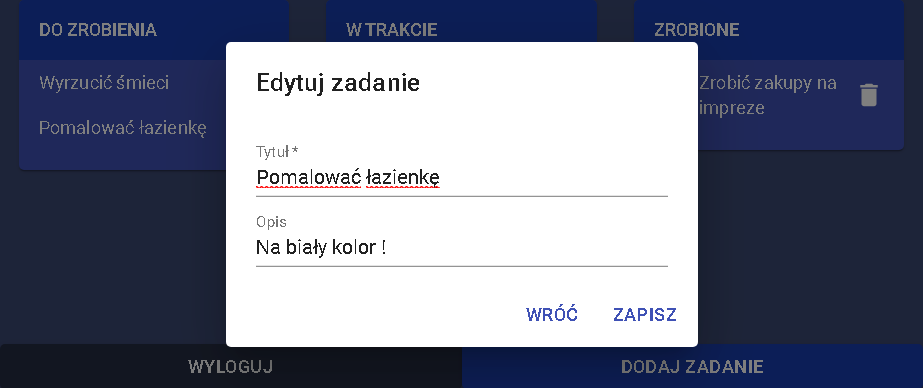
\includegraphics[keepaspectratio,scale=0.5]{./img/edit.PNG} \\
		\subsubsection{Brak połączenia lub nieprzewidziana akcja}
		Podczas utraty połączenia z internetem użytkownik zostanie poproszony o restart aplikacji. \\
		Ten sam komunikat zostanie wyświetlony jeśli użytkownik wykona nieprzewidzianą akcje. \\
		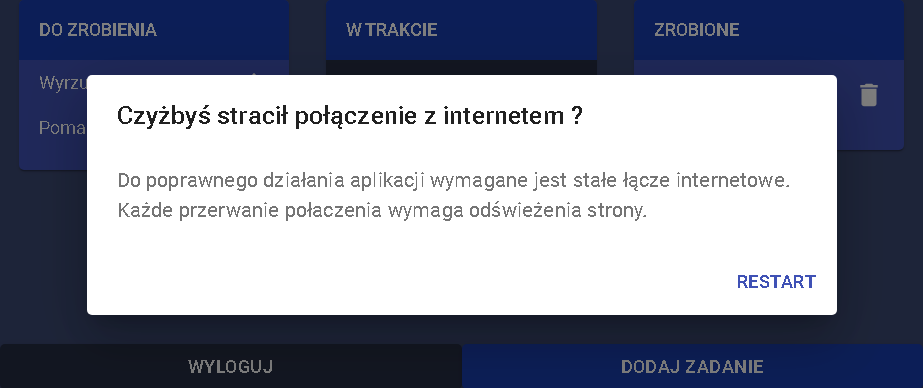
\includegraphics[keepaspectratio,scale=0.5]{./img/error.PNG} \\
	\newpage
	\section{Wykorzystane technologie}
		\subsection{Informacje ogólne}
		Projekt został w wiekszości wykonany przy użyciu języka JavaScript z uwagi na możliwość wykorzystania go po stronie klienta jak i serwera. \\
		Ciekawym aspektem pojektu jest wykorzystanie technologii WebSocket co pozwoliło na aktualizacje danych głownego panelu w czasie rzeczywistym. \\
		Projekt został podzielony na dwa oddzielne podprojekty zwane\\ „mikroserwisami”.\\
		Aplikacje klienta jako jeden serwis posiadającą logike tworzącą interfejs\\ graficzny.\\
		Aplikację serwerową pozwalajaca na komunikacje z interfejsem graficznym jak i logike przechowywania i przetwarzania danych.
		\subsection{Serwer}
		Serwer wykorzystuje następujące technologie:
		\begin{itemize}  
			\item node - platforma uruchomieniowa
			\item express - serwer http
			\item ws - serwer WebSocket
			\item mongodb - baza danych typu noSQL
			\item JSON Web Token - technologia tworzenia tokenów dostępu
		\end{itemize}
		Node pozwala na uruchomienie kodu JavaScript. \\
		Serwer http zapewnia funkcjonalności logowania i rejestracji.\\
		Serwer WebSocket zapewnia wszystkie funkcjonalności związane \\ z zarządzaniem „zadaniami domowymi”. \\
		Baza danych przechowuje informacje dotyczace zarejestrowanych\\ użytkowników oraz „zadań domowych”. \\
		JSON Web Token posiada w sobie logie do tworzenia tokenu pozawalającego na autoryzacje akcji użytwników. \\
		\newpage
		\subsection{Klient}
		\begin{itemize}  
			\item React - framework do tworzenia interfejsów graficznych
			\item React-Redux - biblioteka ułatwiająca trzymanie stan aplikacji
			\item Material UI - bibliotegka z gotwowymi komponentami
			\item Axios - biblioteka do XMLHttpRequests
		\end{itemize}
		Dzięki „React” i „React-Redux” aplikacja została napisana w sposób\\ ustrukturyzowany podzielony na komponenty przez co zwiększyła się\\ czytelność kodu. \\
		Material UI dostarczył wiele gotówych komponentów graficznych\\ zaskutkowało to zwiększeniem tępa pracy jak i samej estetyki. \\
		Axios znacznie ułatwił prace z API serwera przez opakowanie zapytań w „Promise”.
	\section{API servera}
	\subsection{Opis}
	Serwer posiada wiele możliwośći komunikacji. \\
	Część autoryzacji wykorzsystującą protokół http oraz logike do przetwarzania „zadań domowych” wykorzsystująca protokół WebSocket. \\
	Serwer działa nieależnie od klienta przez co możliwe jest napisanie kopletnie innego interfejsu graficznego. \\
	Opisane w tym rodziale API dostarczy wszelkich niezbędnych informacji do prawidłowego odpytywania serwera.
	\subsection{HTTP}
	Główny adress \url{http://housework-api.herokuapp.com/} będę oznaczał \\ jako root. \\
	Wszystkie zapytanią powinny być typu JSON. \\
	Zatem nagłówki zapytań muszą posiadać: 'Content-Type': 'application/json'
	\newpage
	\subsubsection{Rejestracja} 
	\fcolorbox{blue}{myLightBlue}{
		\colorbox{myBlue}{\textcolor{white}{POST}}
		\textcolor{black}{root/user/register}
	}
	
\begin{flushleft}
\textbf{Zapytanie:}
\begin{verbatim}
{
  name: „nazwa użytkownika”,
  password: „hasło użytkownika”
}
\end{verbatim}
\textbf{Odpowiedź:}

Poprawna:
\begin{verbatim}
{
  auth: true,
  token: „token potrzebny do autoryzacji”
}
\end{verbatim}

Błąd:
\begin{verbatim}
{
  auth: false,
  message: „przyczyna błędu”
}
\end{verbatim}
\end{flushleft}

\newpage

	\subsubsection{Logowanie} 
\fcolorbox{blue}{myLightBlue}{
	\colorbox{myBlue}{\textcolor{white}{POST}}
	\textcolor{black}{root/user/login}
}

\begin{flushleft}
	\textbf{Zapytanie:}
	\begin{verbatim}
	{
	name: „nazwa użytkownika”,
	password: „hasło użytkownika”
	}
	\end{verbatim}
	\textbf{Odpowiedź:}
	
	Poprawna:
	\begin{verbatim}
	{
	auth: true,
	token: „token potrzebny do autoryzacji”
	}
	\end{verbatim}
	
	Błąd:
	\begin{verbatim}
	{
	auth: false,
	message: „przyczyna błędu”
	}
	\end{verbatim}
\end{flushleft}
\subsection{WebSocket}
Wszystkie zapytania powinny być typu JSON.\\
Jeżeli dane zapytanie jest błędne serwer w formie odpowiedzi zamknie połączenie.\\

\textbf{Lista wszystkich typów zapytań:}
\begin{itemize}
	\item ping
	\item task\_add
	\item task\_all
	\item task\_move
	\item task\_delete
	\item task\_edit
\end{itemize}

\newpage

\subsubsection{ping}
Protokół WebSocket wymaga systemu pingowania w celu utrzymania połączenia. \\
Następujące zapytanie należy wysyłać do serwera w nie wiekszym odstępnie niz 30 sekund aby połączenie mogło pozostać utrzymane.\\
\begin{flushleft}
\textbf{Zapytanie:}
\begin{verbatim}
{
  type: „ping”
}
\end{verbatim}

\textbf{Odpowiedź:}
\begin{verbatim}
{
  type: „pong”
}
\end{verbatim}
\end{flushleft}
\newpage
\subsubsection{task\_add}
Pozwala na dodanie nowego zadania do bazy \\
\begin{flushleft}
\textbf{Zapytanie:}
\begin{verbatim}
{
  type: „task_add”,
  payload: {
    token: „token”,
    title:„tytuł zadania”,
    description: „opis zadania”,
    timestamp: „timestamp typu JavaScript”
 }
}
\end{verbatim}
\textbf{Odpowiedź:}
\begin{verbatim}
{
  type: „task_add-confirmation”,
  payload: {
  task: „obiekt typy task”
}
\end{verbatim}
\textbf{Broadcast:}
\begin{verbatim}
{
  type: „task_add”,
  payload: {
  task: „taskObiekt”
}
\end{verbatim}
\end{flushleft}
\newpage
\subsubsection{task\_all}
Pozwala na otrzymanie wszystkich zadan znajdujacych sie w bazie \\
\begin{flushleft}
\textbf{Zapytanie:}
\begin{verbatim}
{
  type: „task_all”,
  payload:{
  token: „token”
 }
}
\end{verbatim}
\textbf{Odpowiedź:}
\begin{verbatim}
{
  type: „task_all”,
  payload: [taskObiekt, taskObiekt...]
}
\end{verbatim}
\end{flushleft}
\newpage
\subsubsection{task\_move}
Pozwala na zmienienie pozycji tasku \\
\begin{flushleft}
\textbf{Zapytanie:}
\begin{verbatim}
{
  type: „task_move”,
  payload:{
    token: „token”,
    id: „taskId”,
    position: „TODO” lub „INPROGRESS” lub „DONE”
 }
}
\end{verbatim}
\textbf{Odpowiedź:}
\begin{verbatim}
{
  type: „task_move-confirmation”,
  payload: {
    task: „taskObject”
 }
}
\end{verbatim}
\textbf{Broadcast:}
\begin{verbatim}
{
  type: „task_move”,
  payload: {
    task: „taskObject”
 }
}
\end{verbatim}
\end{flushleft}
\newpage
\subsubsection{task\_delete}
Pozwala na usunięcie zadania \\
\begin{flushleft}
\textbf{Zapytanie:}
\begin{verbatim}
{
  type: „task_delete”,
  payload: {
    token: token,
    id: „TASK ID”,
 }
}
\end{verbatim}
\textbf{Odpowiedź:}
\begin{verbatim}
{
  type: „task_delete-confirmation”,
  payload: {
    task: „taskObject”
 }
}
\end{verbatim}
\textbf{Broadcast:}
\begin{verbatim}
{
  type: „task_delete”,
  payload: {
    task: „taskObject”
  }
}
\end{verbatim}
\end{flushleft}
\newpage
\subsubsection{task\_edit}
Pozwala na edycje zadania \\
\begin{flushleft}
\textbf{Zapytanie:}
\begin{verbatim}
{
  type: „task_edit”,
  payload: {      
    token: „token”,
    id: „taskId”,
    title: „tytuł”,
    description: „opis”
 }
}
\end{verbatim}
\textbf{Odpowiedź:}
\begin{verbatim}
{
  type: „task_edit-confirmation”,
  payload: {
   task: ”taskObject”
  }
}
\end{verbatim}
\textbf{Broadcast:}
\begin{verbatim}
{
  type: „task_edit”,
  payload: {
    task: ”taskObject”
 }
}
\end{verbatim}
\end{flushleft}

\end{document}